\section{Lectrure des propriétés d'une fonction à partir d'un tableau de variation}

On donne ci-dessous les variations d'une fonction $f$, définie et dérivable sur $[-10;20]$, et on nomme $\mathcal{C}$ sa représentation graphique dans un repère orthonormal $(O, \vec{i}, \vec{j})$ :

Répondre par $VRAI$ ou $FAUX$, aux questions suivantes (une justification est demandée lorsque la réponse est $FAUX$, aucune justification n'est demandée lorsque la réponse est $VRAI$).

\begin{center}
	\begin{tikzpicture}[scale=0.8]
		\tkzTabInit{$x$/1.5,$f(x)$/4}{$-10$, $0$, $4$, $9$, $20$}
		%\tkzTabLine { ,+ ,z , -, }
		\tkzTabVar{+/$10$,-/$-2$,+/$3$,-/$-1$,+/$0$}
	\end{tikzpicture}
\end{center}

\begin{questions}
	\question[1]  Pour tout réel $x$, $f(x) \ge -2$.
	\begin{solution}
		FAUX, on ne connaît la fonction $f$ que sur $[-10;20]$ pas sur $\mathbb{R}$.
	\end{solution}
	\question[1]  L'équation $f(x)=-3$ admet au moins une solution dans $[-10;20]$.
	\begin{solution}
		FAUX, dans $[-10;20]$ le minimum de $f$ est $-2$.
	\end{solution}
	\question[1] L'équation $f(x)=1$ admet une solution unique dans $[4;9]$.
	\begin{solution}
		VRAI
	\end{solution}
	\question[1] Pour tout réel $x$, $f'(x)\ge 0$.
	 \begin{solution}
	 	FAUX, sur $[-10;0]$, la fonction $f$ est décroissante, donc $f'(x) \le 0$.
	 \end{solution}
	\question[1] $f'(1)<0$.
	\begin{solution}
		FAUX, sur $[0;4]$, la fonction $f$ est croissante, donc $f'(x)\ge 0$, d'pù $f'(1) \ge 0$
	\end{solution}
\end{questions}